
\documentclass[a4paper,12pt]{article}
%%%%%%%%%%%%%%%%%%%%%%%%%%%%%%%%%%%%%%%%%%%%%%%%%%%%%%%%%%%%%%%%%%%%%%%%%%%%%%%%%%%%%%%%%%%%%%%%%%%%%%%%%%%%%%%%%%%%%%%%%%%%%%%%%%%%%%%%%%%%%%%%%%%%%%%%%%%%%%%%%%%%%%%%%%%%%%%%%%%%%%%%%%%%%%%%%%%%%%%%%%%%%%%%%%%%%%%%%%%%%%%%%%%%%%%%%%%%%%%%%%%%%%%%%%%%
\usepackage{graphicx,hyperref,mathpple,amsmath,exscale,setspace,xcolor}
\usepackage[left=20mm,right=20mm,top=20mm,bottom=20mm]{geometry}
\usepackage{pdflscape,showkeys,changepage}
\usepackage[round]{natbib}

\setcounter{MaxMatrixCols}{15}
%TCIDATA{OutputFilter=LATEX.DLL}
%TCIDATA{Version=5.50.0.2953}
%TCIDATA{<META NAME="SaveForMode" CONTENT="2">}
%TCIDATA{BibliographyScheme=BibTeX}
%TCIDATA{Created=Wednesday, May 03, 2023 13:45:06}
%TCIDATA{LastRevised=Thursday, October 26, 2023 15:04:30}
%TCIDATA{<META NAME="GraphicsSave" CONTENT="32">}
%TCIDATA{<META NAME="DocumentShell" CONTENT="Standard LaTeX\Blank - Standard LaTeX Article">}
%TCIDATA{CSTFile=40 LaTeX article.cst}

\let\oldref\ref
\AtBeginDocument{
\let\oldref\ref\renewcommand{\ref}[1]{(\oldref{#1})}
\newcommand{\bsq}{\begin{subequations}}\newcommand{\esq}{\end{subequations}}
\newcommand{\bls}{\begin{landscape}}\newcommand{\els}{\end{landscape}}
\renewcommand\showkeyslabelformat[1]{{\parbox[t]{\marginparwidth}{\raggedright\footnotesize\url{#1}}}}
\newcommand{\intxt}[1]{\intertext{#1}}\newcommand{\BAW}[1]{\begin{adjustwidth}{-#1mm}{-5mm}}\newcommand{\EAW}{\end{adjustwidth}}
\newcommand{\vsp}[1]{\vspace*{#1mm}}\newcommand{\hsp}[1]{\hspace*{#1mm}}  }
\makeatletter
\renewcommand*{\@fnsymbol}[1]{\ensuremath{\ifcase#1\or *\or
    \#\or \star\or \bowtie\or \star\star\or \ddagger\ddagger \else\@ctrerr\fi}}
\makeatother
\allowdisplaybreaks
\IfFileExists{C:/swp55/TCITeX/TeX/LaTeX/SWmacros/tcilatex.tex}{\input{tcilatex}}{}
\graphicspath{{../graphics/}{graphics/}}
\newcommand{\dble}{1.77}
\newcommand{\sngl}{1.23}
\definecolor{myred}{rgb}{.50,.10,.10}
\definecolor{mygrn}{rgb}{.10,.35,.10}
\definecolor{myblu}{rgb}{.10,.10,.35}
\hypersetup{colorlinks,citecolor=myblu,filecolor=mygrn,linkcolor=myred,urlcolor=mygrn,breaklinks=true}
\setstretch{\sngl}

\begin{document}


\section{MR17 with Monetary policy rule}

Adding a Monetary Policy (MP)\ rule to McCririck and Rees (2017, MR17)
yields to:%
\begin{align}
\tilde{y}_{t}& =a_{y,1}\tilde{y}_{t-1}+a_{y,2}\tilde{y}_{t-2}-\frac{a_{r}}{2}%
\sum_{i=1}^{2}(r_{t-i}-r_{t-i}^{\ast })+\sigma _{1}\varepsilon _{1t}
\label{MR1} \\
\pi _{t}& =(1-\beta _{1})\pi _{t}^{e}+\frac{\beta _{1}}{3}\sum_{i=1}^{3}\pi
_{t-i}+\beta _{2}(u_{t-1}-u_{t-1}^{\ast })+\sigma _{2}\varepsilon _{2t}
\label{MR2} \\
\Delta z_{t}& =\sigma _{3}\varepsilon _{3t},  \label{MR3} \\
\Delta y_{t}^{\ast }& =g_{t}+\sigma _{4}\varepsilon _{4t}\qquad (\text{MR17
use }g_{t}\text{ in paper, we use }g_{t-1}\text{ as in LW03 in SSM below})
\label{MR4} \\
\Delta g_{t}& =\sigma _{5}\varepsilon _{5t}  \label{MR5} \\
\Delta u_{t}^{\ast }& =\sigma _{6}\varepsilon _{6t}  \label{MR6} \\
u_{t}& =u_{t}^{\ast }+\beta (.4\tilde{y}_{t}+.3\tilde{y}_{t-1}+.2\tilde{y}%
_{t-2}+.1\tilde{y}_{t-3})+\sigma _{7}\varepsilon _{7t}  \label{MR7} \\
r_{t}& =(1-b_{1})(r_{t-1}-\Delta \pi _{t})+b_{1}\left[ r_{t}^{\ast }-\bar{\pi%
}-2(u_{t}-u_{t}^{\ast })\right] -\Delta _{2}u_{t}+\sigma _{8}\varepsilon
_{8t},  \label{MR8}
\end{align}%
where $\tilde{y}_{t}=(y_{t}-y_{t}^{\ast })$ and $r_{t}^{\ast }=4g_{t}+z_{t}$
as before, and \ref{MR8} is obtained from the MARTIN policy model of the
Reserve Bank of Australia (Ballantyne \emph{et al.}, 2020), with nominal
rule:%
\begin{equation}
i_{t}=(1-b_{1})i_{t-1}+b_{1}(r_{t}^{\ast }+{\color{red}{2}}\pi _{t}-\bar{\pi}%
-2(u_{t}-u_{t}^{\ast }))-\Delta _{2}u_{t}+\sigma _{8}\varepsilon _{8t},
\label{eq:NR}
\end{equation}%
where $\bar{\pi}$ denotes the inflation target (there is a {\color{red}{2}}
missing in front of $\pi _{t}$ in our equation see below eq. 36 from
Ballantyne \emph{et al.}, 2020). The parameters in \ref{MR8} and \ref{eq:NR}
are:$\ b_{1}=.3$ and $\sigma _{8}=1.19$\ (where is 1.19 taken from???).
These are from the equation below (page 237):

\begin{figure}[h]
\centering
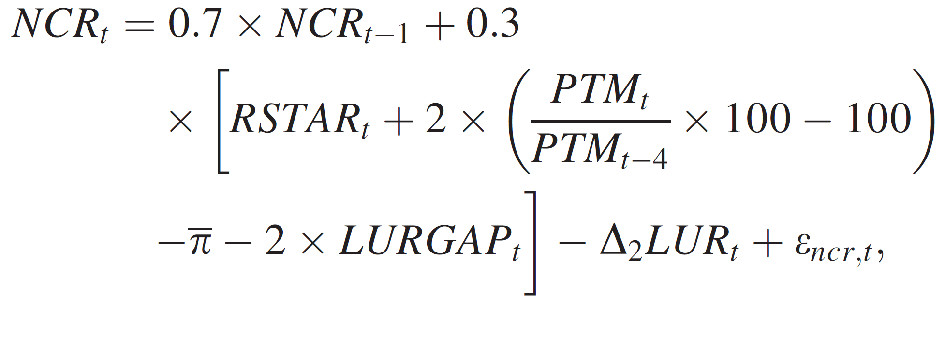
\includegraphics[width=.5\textwidth]{S34R0D00__1}
\end{figure}

\noindent TIM:\ Why use $r_{t}=i_{t}+\pi _{t}$ and not $r_{t}=i_{t}+\pi
_{t}^{e}$, $\Rightarrow $ inconsistent within same model? Also not sure if
the equations are correct... but for shock recovery, all that matters is $%
r_{t}^{\ast }$ and $u_{t}^{\ast }$

The numbered shock to named shock mapping is:
\begin{equation}
\begin{bmatrix}
\varepsilon _{1t} \\
\varepsilon _{2t} \\
\varepsilon _{3t} \\
\varepsilon _{4t} \\
\varepsilon _{5t} \\
\varepsilon _{6t} \\
\varepsilon _{7t} \\
\varepsilon _{8t}%
\end{bmatrix}%
=%
\begin{bmatrix}
\varepsilon _{t}^{\tilde{y}} \\
\varepsilon _{t}^{\pi } \\
\varepsilon _{t}^{z} \\
\varepsilon _{t}^{y^{\ast }} \\
\varepsilon _{t}^{g} \\
\varepsilon _{t}^{u^{\ast }} \\
\varepsilon _{t}^{u} \\
\varepsilon _{t}^{r}%
\end{bmatrix}%
.
\end{equation}

\section{Shock recovery SSM}

\subsection{SSM with lagged states}

Kurz's (2018) SSM has the following general from:\bsq\label{SSM}%
\begin{align}
\mathsf{Measurement}& :\quad Z_{t}=D_{1}X_{t}+D_{2}X_{t-1}+R\varepsilon _{t}
\label{ssm1} \\
\mathsf{State}& :\quad X_{t}=AX_{t-1}+C\varepsilon _{t},  \label{ssm2}
\end{align}%
\esq where $\varepsilon _{t}\sim MN(0,I_{m})$, $D_{1},D_{2},A,R$ are $C$ are
conformable system matrices, $Z_{t}$ the observed variable and $X_{t}$ the
latent state variable.

\subsection{MR17 SSM for shock recovery}

To assess recovery, re-write the model in `\emph{shock recovery}' form. That
is, collect all observables in $Z_{t}$, and all shocks (and other state
variables)\ in state vector $X_{t}$.\bsq\label{ssm0}%
\begin{align}
\mathsf{Measurement}& :\;\quad Z_{1t}=y_{t}^{\ast }-a_{y,1}y_{t-1}^{\ast
}-a_{y,2}y_{t-2}^{\ast }-\frac{a_{r}}{2}\left( r_{t-1}^{\ast }+r_{t-2}^{\ast
}\right) +\sigma _{1}\varepsilon _{1t} \\
\phantom{\mathsf{Measurement}}& \,\,\;\;\phantom{:\quad}Z_{2t}=-\beta
_{2}u_{t-1}^{\ast }+\sigma _{2}\varepsilon _{2t} \\
\phantom{\mathsf{Measurement}}& \,\,\;\;\phantom{:\quad}Z_{3t}=u_{t}^{\ast
}-\beta (.4y_{t}^{\ast }+.3y_{t-1}^{\ast }+.2y_{t-2}^{\ast }+.1y_{t-3}^{\ast
})+\sigma _{7}\varepsilon _{7t} \\
\phantom{\mathsf{Measurement}}& \,\,\;\;\phantom{:\quad}Z_{4t}=b_{1}r_{t}^{%
\ast }+2b_{1}u_{t}^{\ast }+\sigma _{8}\varepsilon _{7t} \\
\mathsf{State}& :\quad \Delta y_{t}^{\ast }=g_{t-1}+\sigma _{4}\varepsilon
_{4t} \\
\phantom{\mathsf{State}}& \;\,\;\phantom{:\quad}\Delta g_{t}=\sigma
_{5}\varepsilon _{5t} \\
\phantom{\mathsf{State}}& \;\,\;\phantom{:\quad}\Delta u_{t}^{\ast }=\sigma
_{6}\varepsilon _{6t},  \label{drstar2} \\
\phantom{\mathsf{State}}& \;\,\;\phantom{:\quad}\Delta r_{t}^{\ast }=4\sigma
_{5}\varepsilon _{5t}+\sigma _{3}\varepsilon _{3t},
\end{align}%
\esq with the observables $Z_{t}$ in the measurement equations defined as:%
\vsp{-3}\bsq\label{ssmO}
\begin{align}
Z_{1t}& =y_{t}-\left( \sum_{i=1}^{2}(a_{y,i}y_{t-i})-\frac{a_{r}}{2}%
\sum_{i=1}^{2}r_{t-i}\right)  \\
Z_{2t}& =\pi _{t}-\left( (1-\beta _{1})\pi _{t}^{e}+\frac{\beta _{1}}{3}%
\sum_{i=1}^{3}\pi _{t-i}+\beta _{2}u_{t-1}\right)  \\
Z_{3t}& =u_{t}-\beta (.4y_{t}+.3y_{t-1}+.2y_{t-2}+.1y_{t-3}) \\
Z_{4t}& =r_{t}-(1-b_{1})(r_{t-1}-\Delta \pi _{t})-b_{1}\bar{\pi}+\Delta
_{2}u_{t}+2b_{1}u_{t}
\end{align}%
\esq

The `\emph{shock recovery}' SSF\ corresponding to \ref{ssm0} is then: \bsq%
\label{K0SSM}\BAW{20}\pagebreak

\begin{align}
\mathsf{Measurement}& :\quad Z_{t}=D_{1}X_{t}+D_{2}X_{t-1}+R\varepsilon _{t}
\notag \\[-4mm]
\underbrace{\left[
\begin{array}{c}
Z_{1t} \\
Z_{2t} \\
Z_{3t} \\
Z_{4t}%
\end{array}%
\right] }_{Z_{t}}& =\underbrace{%
\begin{bmatrix}
1 & -a_{y,1} & -a_{y,2} & 0 & 0 & 0 & 0 & \sigma _{1} & 0 & 0 & 0 & 0 & 0 & 0
& 0 \\
0 & 0 & 0 & 0 & 0 & 0 & 0 & 0 & \sigma _{2} & 0 & 0 & 0 & 0 & 0 & 0 \\
-.4\beta  & -.3\beta  & -.2\beta  & 0 & 0 & 0 & 1 & 0 & 0 & 0 & 0 & 0 & 0 &
\sigma _{7} & 0 \\
0 & 0 & 0 & 0 & b_{1} & 0 & 2b_{1} & 0 & 0 & 0 & 0 & 0 & 0 & 0 & \sigma _{8}%
\end{bmatrix}%
}_{D_{1}}\underbrace{\left[
\begin{array}{c}
y_{t}^{\ast } \\
y_{t-1}^{\ast } \\
y_{t-2}^{\ast } \\
g_{t} \\
r_{t}^{\ast } \\
r_{t-1}^{\ast } \\
u_{t}^{\ast } \\
\varepsilon _{1t} \\
\varepsilon _{2t} \\
\varepsilon _{3t} \\
\varepsilon _{4t} \\
\varepsilon _{5t} \\
\varepsilon _{6t} \\
\varepsilon _{7t} \\
\varepsilon _{8t}%
\end{array}%
\right] }_{X_{t}} \\
& +\underbrace{%
\begin{bmatrix}
0 & 0 & 0 & 0 & -\frac{a_{r}}{2} & -\frac{a_{r}}{2} & 0 & 0 & 0 & 0 & 0 & 0
& 0 & 0 & 0 \\
0 & 0 & 0 & 0 & 0 & 0 & -\beta _{2} & 0 & 0 & 0 & 0 & 0 & 0 & 0 & 0 \\
0 & 0 & -.1\beta  & 0 & 0 & 0 & 0 & 0 & 0 & 0 & 0 & 0 & 0 & 0 & 0 \\
0 & 0 & 0 & 0 & 0 & 0 & 0 & 0 & 0 & 0 & 0 & 0 & 0 & 0 & 0%
\end{bmatrix}%
}_{D_{2}}\underbrace{\left[
\begin{array}{c}
y_{t-1}^{\ast } \\
y_{t-2}^{\ast } \\
y_{t-3}^{\ast } \\
g_{t-1} \\
r_{t-1}^{\ast } \\
r_{t-2}^{\ast } \\
u_{t-1}^{\ast } \\
\varepsilon _{1t-1} \\
\varepsilon _{2t-1} \\
\varepsilon _{3t-1} \\
\varepsilon _{4t-1} \\
\varepsilon _{5t-1} \\
\varepsilon _{6t-1} \\
\varepsilon _{7t-1} \\
\varepsilon _{8t-1}%
\end{array}%
\right] }_{X_{t-1}}+\underbrace{\boldsymbol{0}_{2\times 5}}_{R}\underbrace{%
\begin{bmatrix}
\varepsilon _{1t} \\
\varepsilon _{2t} \\
\varepsilon _{3t} \\
\varepsilon _{4t} \\
\varepsilon _{5t} \\
\varepsilon _{6t} \\
\varepsilon _{7t} \\
\varepsilon _{8t}%
\end{bmatrix}%
}_{\varepsilon _{t}} \\
\mathsf{State}:\quad X_{t}& =AX_{t-1}+C\varepsilon _{t},  \notag \\[5mm]
\underbrace{\left[
\begin{array}{c}
y_{t}^{\ast } \\
y_{t-1}^{\ast } \\
y_{t-2}^{\ast } \\
g_{t} \\
r_{t}^{\ast } \\
r_{t-1}^{\ast } \\
u_{t}^{\ast } \\
\varepsilon _{1t} \\
\varepsilon _{2t} \\
\varepsilon _{3t} \\
\varepsilon _{4t} \\
\varepsilon _{5t} \\
\varepsilon _{6t} \\
\varepsilon _{7t} \\
\varepsilon _{8t}%
\end{array}%
\right] }_{X_{t}}& =\underbrace{%
\begin{bmatrix}
1 & 0 & 0 & 1 & 0 & 0 & 0 & 0 & 0 & 0 & 0 & 0 & 0 & 0 & 0 \\
1 & 0 & 0 & 0 & 0 & 0 & 0 & 0 & 0 & 0 & 0 & 0 & 0 & 0 & 0 \\
0 & 1 & 0 & 0 & 0 & 0 & 0 & 0 & 0 & 0 & 0 & 0 & 0 & 0 & 0 \\
0 & 0 & 0 & 1 & 0 & 0 & 0 & 0 & 0 & 0 & 0 & 0 & 0 & 0 & 0 \\
0 & 0 & 0 & 0 & 1 & 0 & 0 & 0 & 0 & 0 & 0 & 0 & 0 & 0 & 0 \\
0 & 0 & 0 & 0 & 1 & 0 & 0 & 0 & 0 & 0 & 0 & 0 & 0 & 0 & 0 \\
0 & 0 & 0 & 0 & 0 & 0 & 1 & 0 & 0 & 0 & 0 & 0 & 0 & 0 & 0 \\
0 & 0 & 0 & 0 & 0 & 0 & 0 & 0 & 0 & 0 & 0 & 0 & 0 & 0 & 0 \\
0 & 0 & 0 & 0 & 0 & 0 & 0 & 0 & 0 & 0 & 0 & 0 & 0 & 0 & 0 \\
0 & 0 & 0 & 0 & 0 & 0 & 0 & 0 & 0 & 0 & 0 & 0 & 0 & 0 & 0 \\
0 & 0 & 0 & 0 & 0 & 0 & 0 & 0 & 0 & 0 & 0 & 0 & 0 & 0 & 0 \\
0 & 0 & 0 & 0 & 0 & 0 & 0 & 0 & 0 & 0 & 0 & 0 & 0 & 0 & 0 \\
0 & 0 & 0 & 0 & 0 & 0 & 0 & 0 & 0 & 0 & 0 & 0 & 0 & 0 & 0 \\
0 & 0 & 0 & 0 & 0 & 0 & 0 & 0 & 0 & 0 & 0 & 0 & 0 & 0 & 0 \\
0 & 0 & 0 & 0 & 0 & 0 & 0 & 0 & 0 & 0 & 0 & 0 & 0 & 0 & 0%
\end{bmatrix}%
}_{A}\underbrace{\left[
\begin{array}{c}
y_{t-1}^{\ast } \\
y_{t-2}^{\ast } \\
y_{t-3}^{\ast } \\
g_{t-1} \\
r_{t-1}^{\ast } \\
r_{t-2}^{\ast } \\
u_{t-1}^{\ast } \\
\varepsilon _{1t-1} \\
\varepsilon _{2t-1} \\
\varepsilon _{3t-1} \\
\varepsilon _{4t-1} \\
\varepsilon _{5t-1} \\
\varepsilon _{6t-1} \\
\varepsilon _{7t-1} \\
\varepsilon _{8t-1}%
\end{array}%
\right] }_{X_{t-1}}+\underbrace{%
\begin{bmatrix}
0 & 0 & 0 & \sigma _{4} & 0 & 0 & 0 & 0 \\
0 & 0 & 0 & 0 & 0 & 0 & 0 & 0 \\
0 & 0 & 0 & 0 & 0 & 0 & 0 & 0 \\
0 & 0 & 0 & 0 & \sigma _{5} & 0 & 0 & 0 \\
0 & 0 & \sigma _{3} & 0 & 4\sigma _{5} & 0 & 0 & 0 \\
0 & 0 & 0 & 0 & 0 & 0 & 0 & 0 \\
0 & 0 & 0 & 0 & 0 & \sigma _{6} & 0 & 0 \\
1 & 0 & 0 & 0 & 0 & 0 & 0 & 0 \\
0 & 1 & 0 & 0 & 0 & 0 & 0 & 0 \\
0 & 0 & 1 & 0 & 0 & 0 & 0 & 0 \\
0 & 0 & 0 & 1 & 0 & 0 & 0 & 0 \\
0 & 0 & 0 & 0 & 1 & 0 & 0 & 0 \\
0 & 0 & 0 & 0 & 0 & 1 & 0 & 0 \\
0 & 0 & 0 & 0 & 0 & 0 & 1 & 0 \\
0 & 0 & 0 & 0 & 0 & 0 & 0 & 1%
\end{bmatrix}%
}_{C}\underbrace{%
\begin{bmatrix}
\varepsilon _{1t} \\
\varepsilon _{2t} \\
\varepsilon _{3t} \\
\varepsilon _{4t} \\
\varepsilon _{5t} \\
\varepsilon _{6t} \\
\varepsilon _{7t} \\
\varepsilon _{8t}%
\end{bmatrix}%
}_{\varepsilon _{t}}
\end{align}%
\EAW\esq

\subsubsection{Correlation between true change in natural rate and estimate}

The correlation between the true and estimated $\Delta r_{t}^{\ast }$ from
the SSM can be constructed from the relation:%
\begin{equation}
\rho =0.5\frac{\mathrm{Var}(\Delta r_{t}^{\ast })+\mathrm{Var}(E_{T}\Delta
r_{t}^{\ast })-\phi }{\sigma (\Delta r_{t}^{\ast })\sigma (E_{T}\Delta
r_{t}^{\ast })},
\end{equation}
where $\mathrm{Var}(\Delta r_{t}^{\ast })=4^{2}c^{2}\sigma _{5}^{2}+\sigma
_{3}^{2}$, $\sigma (\Delta r_{t}^{\ast })=\sqrt{\mathrm{Var}(\Delta
r_{t}^{\ast })}$, and $\mathrm{Var}(E_{T}\Delta r_{t}^{\ast })$ can be
computed from simulating from the true model, applying the Kalman Filter and
Smoother to get $E_{T}\Delta r_{t}^{\ast }$ and then computing the sample
variance of $E_{T}\Delta r_{t}^{\ast }$ as an estimate of $\mathrm{Var}%
(E_{T}\Delta r_{t}^{\ast })$.

To obtain $\phi $, add $\Delta r_{t}^{\ast }$ to the state-vector $X_{t}$
and augment the remaining matrices to be conformable. The required $\phi $
term is then the entry of $\mathrm{diag}(P_{t|T}^{\ast })$ that corresponds
to $\Delta r_{t}^{\ast }$, which will be the very last element\ (see also
LW03.pdf how this is done).

\bigskip \pagebreak

\subsection{Check $i_{t}$ to $r_{t}$ conversion}

Ballantyne et al., 2020 equation 36 is something like%
\begin{equation*}
i_{t}=Ai_{t-1}+b_{1}\left[ r_{t}^{\ast }+2\pi _{t}-\bar{\pi}-2\left(
u_{t}-u_{t}^{\ast }\right) \right] -\Delta _{2}u_{t}+\sigma _{8}\varepsilon
_{t}
\end{equation*}%
where $A=(1-b_{1})$. With $i_{t}=r_{t}+\pi _{t}$ (not inflation expectations
as in the model), we get:%
\begin{align}
i_{t}& =Ai_{t-1}+b_{1}2\pi _{t}+\underbrace{b_{1}\left[ r_{t}^{\ast }-\bar{%
\pi}-2\left( u_{t}-u_{t}^{\ast }\right) \right] -\Delta _{2}u_{t}+\sigma
_{8}\varepsilon _{t}}_{OT=~\text{other terms}}  \notag \\
& =Ai_{t-1}+b_{1}2\pi _{t}+OT  \notag \\
\Leftrightarrow (r_{t}+\pi _{t})& =A(r_{t-1}+\pi _{t-1})+2b_{1}\pi _{t}+OT
\notag \\
r_{t}& =Ar_{t-1}+A\pi _{t-1}+2b_{1}\pi _{t}-\pi _{t}+OT  \notag \\
& =Ar_{t-1}+(b_{1}-1)\pi _{t}+A\pi _{t-1}+b_{1}\pi _{t}+OT  \notag \\
& =Ar_{t-1}-(1-b_{1})\pi _{t}+A\pi _{t-1}+b_{1}\pi _{t}+OT  \notag \\
& =Ar_{t-1}-A\pi _{t}+A\pi _{t-1}+b_{1}\pi _{t}+OT  \notag \\
& =Ar_{t-1}-A\Delta \pi _{t}+b_{1}\pi _{t}+OT  \notag \\
& =A(r_{t-1}-\Delta \pi _{t})+b_{1}\pi _{t}+b_{1}\left[ r_{t}^{\ast }-\bar{%
\pi}-2\left( u_{t}-u_{t}^{\ast }\right) \right] -\Delta _{2}u_{t}+\sigma
_{8}\varepsilon _{t}  \notag \\
& =A(r_{t-1}-\Delta \pi _{t})+b_{1}\left[ r_{t}^{\ast }+(\pi _{t}-\bar{\pi}%
)-2\left( u_{t}-u_{t}^{\ast }\right) \right] -\Delta _{2}u_{t}+\sigma
_{8}\varepsilon _{t}  \notag \\
r_{t}& =(1-b_{1})(r_{t-1}-\Delta \pi _{t})+b_{1}\left[ r_{t}^{\ast }+(\pi
_{t}-\bar{\pi})-2\left( u_{t}-u_{t}^{\ast }\right) \right] -\Delta
_{2}u_{t}+\sigma _{8}\varepsilon _{t}
\end{align}

$\Rightarrow $ If the additional $2$ in front of $\left( \frac{PTM_{t}}{%
PTM_{t-4}}\times 100-100\right) $ is intentional.

\bigskip

\bigskip

\end{document}
